\chapter{Analysis}

Now that we have described the game's design, in this chapter, we will explain the approach we took to implement it from a high-level perspective.
We will provide concrete details only for what will be implemented in the playable demo version, but as always, we will make many decisions based on the original vision of our game.

\section{Game Engine}

Game engines provide many important and useful systems for us, so we can focus on implementing the game logic.
For our game, we chose Unity because it offers all the features we need, and the author is already familiar with it.
There are many game engines we could have used, and the high-level decisions presented in this chapter would be still applicable.
However, in some sections we will use nomenclature that is specific to Unity, so we assume the reader is at least familiar with it.
More information is available in the official documentation~\cite{UnityDocs}.

\section{Procedural Generation}\label{sec:analysis-procedural-generation}

As explained in the previous chapter, a lot of the game will be procedurally generated, including the map of a run and each battle along the way.
In the next few sections, we will decide how to generate the worlds for the battles, and in section~\ref{sec:analysis-waves}, we will focus on generating the waves of attackers.

We also want to procedurally generate the map of each run, however the run map will not be a part of the demo version of our game, so we won't implement the map generator yet.
Many of the parameters for the procedurally generated battles will be decided by the map generator.
For example, at the start of each run, the battles should be easy, and they should gradually get more difficult further into the run.
Additionally, some battles will be special in some way.
For example, some battles will be harder, or use a unique terrain type.
We should decide what will be determined by the map generator before the battle generates, and what will be determined only once the battle starts generating.

The map generator will select the terrain type of the world and what attacker types will appear.
These parameters define the theme of the battle.
To control the difficulty, the map generator dictates how difficult should the waves of attackers be, and how much \emph{fuel} is required to finish the level.
This is further explained in section~\ref{sec:analysis-waves}.
The number of attacker path starts and the path lengths also greatly influences the difficulty.
More paths are harder to cover with defenses than a single path.
Shorter paths give the player's defenses less time to deal with the attackers than longer paths.
The map generator will also define the maximum number of path branches, since the paths can split into more.
This is mainly to limit the complexity of the path network in some levels.
There are many more factors which influence the difficulty of the battle, but they are more difficult to quantify, and we believe their influence is not as great.

The worlds the battles take place on are composed of three somewhat distinct parts~--- paths, terrain and obstacles.
It would make the most sense to generate each part separately, one after another.
We should start with the part that is the most restricted, because each part is additionally restricted by what was generated before it.
For this reason, we will start with paths.
There are a lot of rules the paths should follow, as described in section~\ref{sec:design-paths}.
Additionally, the map generator exactly specifies their number, lengths, and maximum number of branches.
So, we will generate paths first (section~\ref{sec:analysis-path-generation}), then the terrain (\ref{sec:analysis-terrain-generation}), and finally, the obstacles (\ref{sec:analysis-obstacles}).

All the randomized algorithms we will use require a source of randomness.
For reasons described in section~\ref{sec:design-procedural-generation}, we need to choose the right random number generator for our use-case.
This is further explained in section~\ref{sec:analysis-rng}.

\section{Path Generation}\label{sec:analysis-path-generation}

In the previous section, we decided that when generating a world, we will start with the paths.
We also mentioned that we will get the number of path starts, their path lengths and the maximum number of branches as an input from the map generator, because these values heavily influence difficulty.
In section~\ref{sec:design-paths}, we outlined many requirements and suggestions for the paths, in order to make them play well.
Generating a path network with good properties is not an easy task.
To simplify it, we can split the path generation process into three simpler problems:
\begin{enumerate}
    \item Select the Hub position and path starts.
    \item Generate the main branch from each path start.
    \item Refine the paths and make them split and join.
\end{enumerate}
How to accomplish the goal of each of these stages will be described in the following subsections of this section.

Before we continue, we would like to define several terms which we'll use in the rest of this section.
These are illustrated in figure~\ref{fig:path-network}.

As stated in section~\ref{sec:design-world}, the world is formed by a $15\times15$ grid of square \textbf{tiles}.
Each tile shares an edge with up to four \textbf{neighboring tiles}, or \textbf{neighbors}.
The outermost tiles of the world which have less than four neighbors are the \textbf{edge tiles}.
The tile the Hub is on is the \textbf{Hub tile}.
Some tiles can be marked as \textbf{path starts}.

A \textbf{path network} consists of \emph{path segments}.
Each \textbf{path segment} is an oriented straight line from the center of one tile to the center of its neighbor.
We can think of them as the edges in an oriented graph, with tiles being the nodes.
A tile with at least one segment starting or ending at it is a \textbf{path tile}.
A \textbf{path} or a \textbf{branch} is a sequence of consecutive segments.
The \textbf{number of extra branches} of a path network could be defined as the sum of the number of outgoing segments from each tile beyond the first.
For example, the path network in figure~\ref{fig:path-network} has 2 path starts and 2 extra branches.

\begin{center}
    \captionsetup{type=figure}
    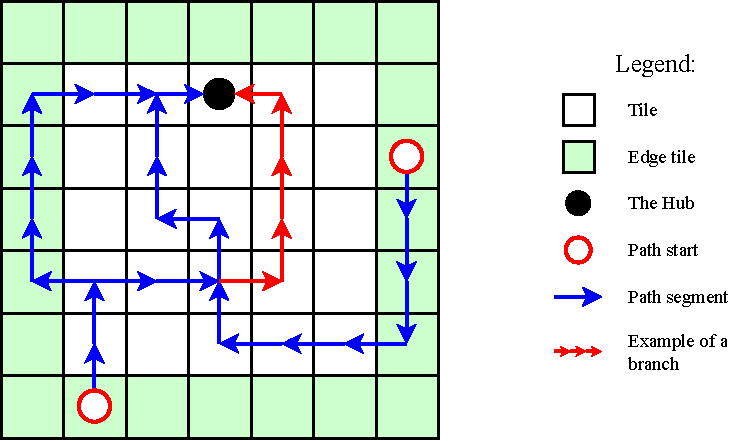
\includegraphics[width=0.7\textwidth]{img/Example path network.pdf}
    \caption{A path network in a $7\times7$ tile world.}
    \label{fig:path-network}
\end{center}

If tile $u$ can be reached from tile $t$ by going along $d$ path segments, we say the \textbf{path distance} from $t$ to $u$ is $d$.
Two tiles can have multiple path distances when multiple paths between them exist.
When $u$ is not reachable from $t$, they do not have a path distance.
The \textbf{path length} of a start dictates its path distance to the Hub.
For example, the path start on the bottom left of figure~\ref{fig:path-network} technically has 3 path distances to the Hub, all of them are 9.
This means its path length is 9.

\subsection{Hub Position and Path Starts} \label{sec:analysis-path-starts}

In the first stage of path generation, we need to select the tile the Hub will be on, and all the path starts.
This will be informed by the number of path starts we have to generate and their path lengths.

First, we will select the Hub tile.
According to requirement RP\ref{RP:hub-pos}, it \enquote{should not be near the edge of the world, and it should be close to the center in levels with multiple paths}.
There aren't any more requirements, so we will simply select a random tile from tiles that are at most some distance from the center using the euclidean metric.
This distance will be the greatest for levels with one path start and decrease with each additional path start.

Now we select the path starts.
According to requirement RP\ref{RP:start-outside}, \enquote{paths start on tiles just outside the playable world, and the first path segment goes from the path start to the nearest tile in the playable world.}
However, other path segments are confined to the actual tiles of the world.
For simplicity, and to avoid edge cases when generating paths, we will pretend, that the paths start at an edge tile of the world, where the first path segment will end.

We will add this segment going over the edge only after the paths are generated.
This segment is uniquely determined anyway, except in the corners of the world, where we'll always select the one that makes the path go straight, as shown in figure~\ref{fig:real-path-starts}.
On the right are the pats as we think of them when generating, and on the left are the actual final paths.
The red circles represent the path starts, and the arrows represent the first segment of each path that only gets added at the end.

\begin{center}
    \captionsetup{type=figure}
    \begin{minipage}{.5\textwidth}
        \centering
        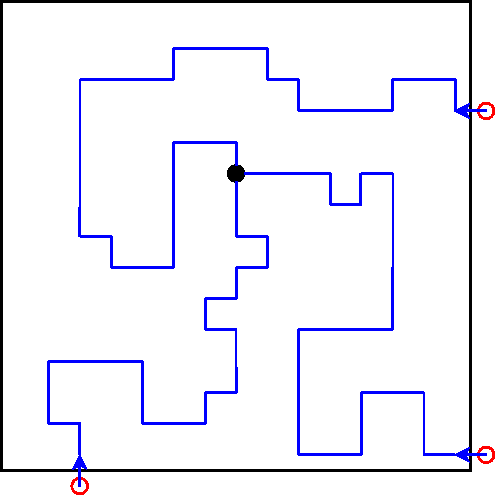
\includegraphics[width=0.95\textwidth]{img/path starts real.pdf}
    \end{minipage}%
    \begin{minipage}{.5\textwidth}
        \centering
        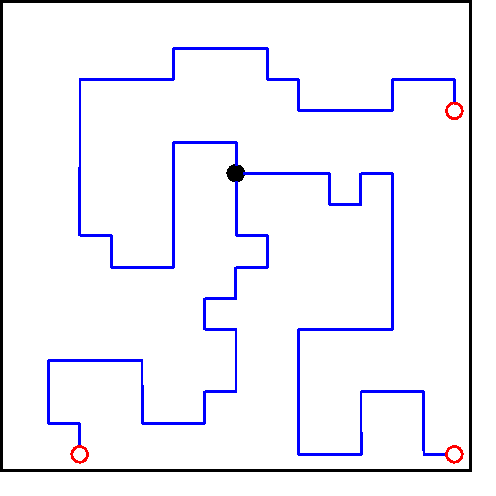
\includegraphics[width=0.95\textwidth]{img/path starts theory.pdf}
    \end{minipage}
    \caption{Real path starts compared to the ones we work with.}
    \label{fig:real-path-starts}
\end{center}

What tiles are valid for a path start with a given path length?
Each start must be at an edge tile, such that a path of the given length can go from it to the Hub.
It is easy to see that the minimum path distance between two tiles is their Manhattan distance.
So, we know that each start cannot be further from the Hub in Manhattan distance that its path length.

We can imagine creating a path backwards from the Hub by appending a segment at every step.
After the first step, the path starts on the neighboring tile of the Hub tile.
Both Manhattan distance and path distance from the tile to the Hub are 1.
After every step, the path distance increases by 1, changing its parity from odd to even or vice versa.
The Manhattan distance to the Hub either increases or decreases by 1, also changing its parity.
Thus, the parity of the path distance and Manhattan distance always match.
This means a path start with an even path length must be a tile with an even Manhattan distance to the Hub, and analogously for odd lengths.

In levels with more paths, we want the path starts to be spread out from each other, in order to cover the world with paths more evenly.
We can choose a minimum distance between the paths starts.
For levels with just one long path, we can also set a minimum distance from the Hub, so it starts further away from it and has more space to zigzag through the world.

To actually select the starts, we find all edge tiles, and separate them into two sets~--- each for one parity.
Then to select each start, we can use rejection sampling.
This means we take random tiles from the set of with the correct parity until we find one that satisfies all the conditions.
As long as the minimum distances between path starts and from the Hub are small enough, this approach always yields a valid list of path starts.
However, with stricter parameters it is possible that the first few starts invalidate all other start positions.
In that case we can use rejection sampling again~--- trying to randomly select lists of starts, until we get one that's valid.
If the failure rate was great enough, it would be wise to select a different algorithm, but our requirements are not very strict, so rejection sampling works fine.

\subsection{Generating the Main Paths}

From the previous step, we have the Hub position and all the path starts.
Now we want to generate the main paths, which will serve as a template for the next steps.
These paths have to have the correct lengths and follow the requirements, which we set in section~\ref{sec:design-paths}.

We couldn't find many resources on procedurally generated paths.
There is a lot of research on generating road networks, mazes or dungeons.
Theoretically, we could use one of the many algorithms for generating mazes~\cite{MazeWiki}, and modify it to suit our needs.
However, it would be difficult to achieve what we need using an approach that was designed for something else.

We found one algorithm specifically designed for procedurally generating paths, called \emph{path chiseling} by Boris the Brave on his blog~\cite{PathChiseling1}\cite{PathChiseling2}.
This algorithm creates random paths on a tile grid by randomly blocking off individual tiles until only one path remains.
This is more promising, however we were unable to find a good way to modify it to generate paths of specific lengths with the properties we want.

Since many of our requirements are more like suggestions, we always want to fulfill them almost the best we can.
This means we can look at the task as an optimization problem: create the \emph{best looking} paths, given the requirements like length, no crossing etc.
Since we want the paths to be randomized, we don't need to find the optimum, we only need a random solution that is good enough.
Given this, we decided to generate the paths using an optimization technique called \emph{simulated annealing}.

\subsection{Simulated Annealing}\label{sec:analysis-simulated-annealing}

Simulated annealing can be used to find an approximation of the global optimum of an optimization problem, much faster than it would take to find the exact global optimum.
A great analysis of this technique can be found in the article \citetitle{SimulatedAnnealing}~\cite{SimulatedAnnealing}.
In this section, we will describe the technique, and in the next section~(\ref{sec:analysis-our-simulated-annealing}), we will use it to generate the paths we want.

The problems simulated annealing can be used for have to be formulated as follows:
\begin{quotation}
    From the set of all states $S$, find a state $s^*$ that minimizes the cost function $f \colon S \to \R$, given a neighbor function $n \colon S \to \mathcal{P}(S)$ which gives the \emph{neighbor states} of each state.
\end{quotation}
For example, to use simulated annealing to solve the \emph{travelling salesman problem}, each state is usually defined as a permutation of the cities to be visited.
The cost function then gives the length of the salesman's path, and the neighbor function gives all the states that can be acquired by swapping two cities in the original state.

The process of simulated annealing is described in pseudocode as algorithm~\ref{alg:simulated-annealing}.
It starts in an initial state $s_0$ and runs for $max\_steps$ steps.
For each step, a temperature $t$ is computed, slowly decreasing from $t_{initial}$ in the first step, to $t_{final}$ at the final step.
In each step, a random neighbor $s'$ of the current state $s$ is selected, and an acceptance probability $p$ is computed, based on the values of $f(s)$, $f(s')$ and the current temperature $t$.
The new state $s'$ is then set as the current state with probability $p$.

This acceptance probability function can be implemented however we see fit, however it should follow these rules:
It always accepts a better new state ($s'$ such that $f(s') < f(s)$), but it can also give a non-zero probability when the new state is worse that the current state ($f(s') > f(s)$).
The probability to accept a worse new state decreases with decreasing temperature.
The acceptance probability of state $t$ cannot be greater than the probability of $u$ when $t$ is worse than $u$ ($f(t) > f(u)$).

\begin{algorithm}[H]
    \caption{Simulated annealing}
    \label{alg:simulated-annealing}
    \begin{algorithmic}[1]
        \State $s \gets s_0$
        \For{$k$ from $0$ to $max\_steps-1$}
        \State $t \gets$ \Call{Lerp}{$t_{initial}$, $t_{final}$, $k/(max\_steps-1)$}
        \State $s' \gets$ random neighbor from $n(s)$
        \State $p \gets$ \Call{AcceptanceProbability}{$f(s)$, $f(s')$, $t$}
        \State with probability $p$: $s \gets s'$
        \EndFor\\
        \Return $s$
        \Statex
    \end{algorithmic}
\end{algorithm}

It is easy to see that if the algorithm never accepted states which are worse than the current state, it would gradually reach a local optimum.
Since it also accepts worse states, it can move away from the local optimum and hopefully end up in a better one.
The probability to accept a worse state gradually decreases with the decreasing temperature.
So at the start, when the temperature is high, the algorithm explores the search space a lot, but as the temperature decreases, it is less and less likely to escape from the local optimum it finds.
Since the exploration prioritizes better states, it is more likely to lead the algorithm to a better optimum than a worse one.

\subsection{Generating Paths using Simulated Annealing}\label{sec:analysis-our-simulated-annealing}

To use simulated annealing to optimize paths, we need to formulate our task as an optimization problem that simulated annealing can solve.
We need to define what is a state, a cost function and a neighbor function.

\head{States}{sa-states}
Each state is a path network composed of one path for each path start.
We will represent each path by a sequence of tiles the path goes through.
Two consecutive tiles in the sequence must be neighbors.
Additionally, each path starts at the given path start, has the correct length, and ends at the Hub tile.
We chose this representation to make it easy to generate neighbor states.
Notice, that we don't check for any intersections and a path can visit one tile multiple times.
This is because the state is going to change only by a small amount at every step.
If we banned intersections, we would lose too much freedom during the simulated annealing, and the final state would always end up close to the initial state.

\head{Neighbor States}{sa-neighbors}
We decided that two states are neighbors when they differ only by one tile.
To generate the set of all neighbors, we have to find all the ways to change one tile in the state to a different tile, such that the result is still a valid state.

For a state to be valid, we require that each path starts with the path start and ends with the Hub tile.
This means that the first and last tile of every path can never change.
For each other tile, there aren't many options on how to change it.
All these options, up to symmetry, are illustrated in figure~\ref{fig:path-tile-swaps}.
The tiles in the sequence are drawn as circles connected by arrows that show their order in the sequence.
The tile we plan to change is drawn as a red circle.
Additionally, we draw the tiles which go before and after it in the sequence.
These are the only tiles that determine the possible changes:
When the tiles form a straight line, no change is possible.
When they form a right angle, one change is possible.
And when the same tile comes before and after, 3 changes are possible.

\begin{center}
    \captionsetup{type=figure}
    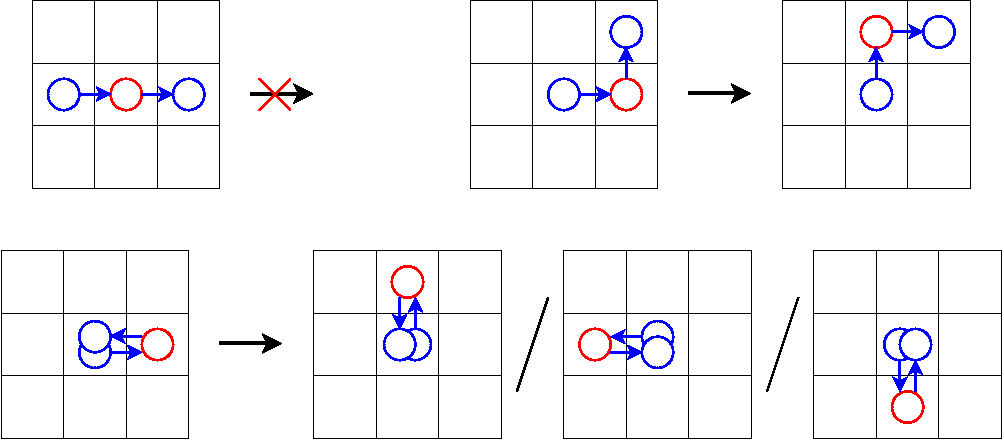
\includegraphics[width=0.7\textwidth]{img/SA tile swaps.pdf}
    \caption{All the possible tile changes.}
    \label{fig:path-tile-swaps}
\end{center}

\head{Cost function}{sa-cost-function}
Now we select a cost function that gives a better score to paths that are more desirable.
Since we want the paths to spread out, we can calculate fore each tile of the world what we call a \emph{crowding penalty}.
Each time a tile appears in the state, it's crowding penalty increments by 1, and all other tiles get a lower penalty decreasing with euclidean distance.
This way, the tiles that get visited the most times get the highest crowding penalty.
A tile can be substantially crowded even when no path goes through it just because there is a lot of paths around it.

We will denote the crowding penalty that tile $t$ gets from tile $u$ as $c(t,u)$.
The total crowding penalty from tiles $c_t(t,s)$ in state $s$ for a given tile $t$ is then $c_t(t,s) = \sum_{u \in s} c(t,u)$.

We also add a big crowding penalty to the tiles along the edge of the world, which gradually decreases as we go away from the edge.
This is to push the paths away from the edges, as that is undesirable by requirement RP\ref{RP:undesirable}.
We will denote the crowding penalty that tile $t$ gets from its closeness to the edge as $c_e(t)$

We define the cost function of a state $s$ as the sum of the crowding penalties of each tile in the state:
\begin{equation*}
    f(s) = \sum_{t \in s} \left(c_e(t) + c_t(t)\right) = \sum_{t \in s} \left(c_e(t) + \sum_{u \in s} c(t,u) \right)
\end{equation*}
This is an obvious choice, because we want each tile to be crowded as little as possible.
So, a state with less crowded tiles has a lower cost, and a state with more crowded tiles has a higher cost.

However, we can just calculate the relative improvement $r_i = f(s) - f(s')$ between the current state $s$ and the new state $s'$ to save on computation.
The relative improvement still gives us enough information to create a good acceptance probability function, but it is simple to compute, because $s$ and $s'$ share most of their tiles.

For $s'$ obtained by changing tile $v$ in $s$ to $w$, we can calculate $r_i$ as
\begin{equation*}
    r_i = c_e(v) - c_e(w)  + 2 c_t(v,s) - 2 c_t(w,s) + 2c(w,v) - 2.
\end{equation*}
We prove this in section~\ref{sec:analysis-proof-improvement}.
This can be computed in $O(1)$ time if we keep the $c_t(t,s)$ of every tile $t$ in the world.
We have to keep all $c_t$ updated when we change the current state to the new state.
This update is simple for each tile $t$:
\begin{equation*}
    c_t(t,s') = c_t(t,s) - c(t,v) + c(t,w).
\end{equation*}

\head{Initial State}{sa-initial-state}
Now, with the problem formulated, we still need to fill in a few details to be able to solve it.
First, we need to produce an initial state.
This is not trivial, because of our constraints on what's considered a valid state.
Namely, every path has to be the correct length.
However, we can easily produce a valid initial state using a random walk from each path start.

The algorithm starts on the path start tile, and adds it to the state as the first path tile of this path.
Then it moves to a random neighbor and appends it to the sequence.
This is repeated until it creates a path of the correct length.
However, we need to ensure that the path ends at the Hub.
To achieve this, we just make the algorithm never select a tile that is further away from the Hub in Manhattan distance, than the remaining length of the path.

\head{Acceptance Probability Function}{sa-acceptance-probability-function}
Next, we need to select an acceptance probability function that works well for this problem.
We don't compute the cost of the current state $f(s)$ and the cost of the new state $f(s')$ separately, instead we compute only the relative improvement $r_i = f(s) - f(s')$.
This means that the function will decide on the probability only based on the relative improvement and the temperature.
The function needs to fulfill the requirements outlined in the previous section~\ref{sec:analysis-simulated-annealing}.
The most straight-forward function is simply $r_i - t$.
This function can return values greater than 1 and less than 0, this does not matter, because when testing the probability, these values get treated as 1, respectively 0.

Is this the best function for this problem?
We don't know, but it performed well in our testing, so we kept it.

\head{Intersection Untwisting}{sa-intersections}
However, when we use simulated annealing with these parameters, it still sometimes produces paths that intersect.
This is because it is difficult for the algorithm to fix a loop in the path, as shown on the left in figure~\ref{fig:untwisting-paths}.
It would first have to bring many path tiles closer together, in order to let them cross over each other.
This is the sort of problem simulated annealing is supposed to be able to overcome.
However, we can help it by adding a step that just \emph{untwists} crossings by reversing the section of the path that forms a loop, as shown in the figure.
This still leaves two identical tiles, but now, simulated annealing can drive these apart without any issue.

\begin{center}
    \captionsetup{type=figure}
    \begin{tikzpicture}
        \draw[step=1.0,black,thin] (0,0) grid (4,4);
        \draw[step=1.0,black,thin] (6,0) grid (10,4);
        \begin{scope}[blue,very thick,decoration={
                        markings,
                        mark=between positions 0.25cm and -0.05cm step 0.5cm with {\arrow{>}};
                    }]
            \draw[postaction={decorate},shift={(0.5,0.5)}] (-1,1)--(3,1);
            \draw[white,line width=4pt,shift={(0.5,0.5)}] (1,0.6)--(1,1.4);
            \draw[postaction={decorate},shift={(0.5,0.5)}] (3,1)--(3,3)--(1,3)--(1,-1);
            \draw[postaction={decorate},shift={(0.5,0.5)}] (5,1)--(6.95,1.05);
            \draw[postaction={decorate},shift={(0.5,0.5)}] (6.95,1.05)--(7,3);
            \draw[postaction={decorate},shift={(0.5,0.5)}] (7,3)--(9,3)--(9,1);
            \draw[postaction={decorate},shift={(0.5,0.5)}] (9,1)--(7.05,0.95);
            \draw[postaction={decorate},shift={(0.5,0.5)}] (7.05,0.95)--(7,-1);
        \end{scope}
        \draw[->,very thick,shift={(0.5,0.5)}] (4,1.5) -- (5,1.5);
    \end{tikzpicture}
    \caption{Untwisting a self-intersecting path.}
    \label{fig:untwisting-paths}
\end{center}

This modification of the state is valid, because the length of the path doesn't change.
However, we cannot untwist crossings between two different paths, because that could change their lengths.
This means that we should take special care to not produce an initial state where two different paths cross.
We can achieve this by calculating crowding penalties when creating the initial state.
Then, when the random walk algorithm selects a random neighbor to move to, we make it prefer the neighbors with a lower crowding penalty.
Because we don't mind self-intersections, we don't add the crowding penalties from the nodes of the path the algorithm is currently creating.
We add them only when the path is complete.

Sill, the algorithm sometimes fails in creating a valid path network.
In case no valid network is generated, we can restart the path generation algorithm, including picking new starting positions.

In figure~\ref{fig:simulated-annealing}, we can see how the paths evolve over time as the temperature decreases.
\begin{center}
    \captionsetup{type=figure}
    \begin{minipage}{.5\textwidth}
        \centering
        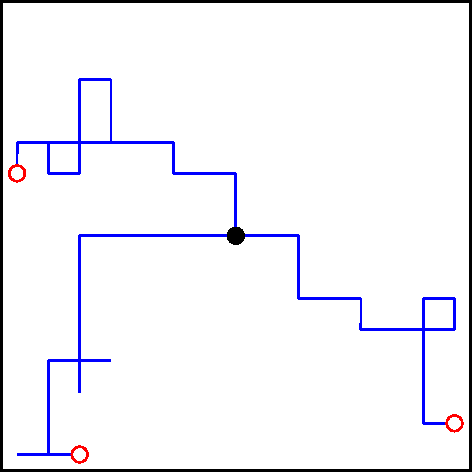
\includegraphics[width=0.95\linewidth]{img/SA initial state.pdf}
        \subcaption{Initial state ($t_{initial} = 2.5$)}
    \end{minipage}%
    \begin{minipage}{.5\textwidth}
        \centering
        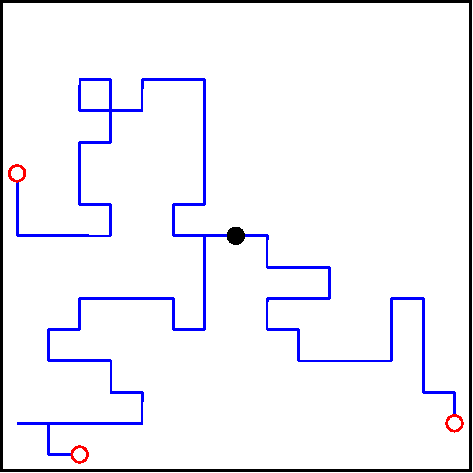
\includegraphics[width=0.95\linewidth]{img/SA temp 2.pdf}
        \subcaption{$t = 2$}
    \end{minipage}\\
    \begin{minipage}{.5\textwidth}
        \centering
        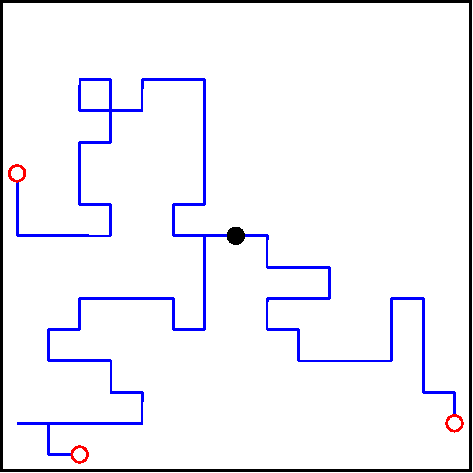
\includegraphics[width=0.95\linewidth]{img/SA temp 1.5.pdf}
        \subcaption{$t = 1.5$}
    \end{minipage}%
    \begin{minipage}{.5\textwidth}
        \centering
        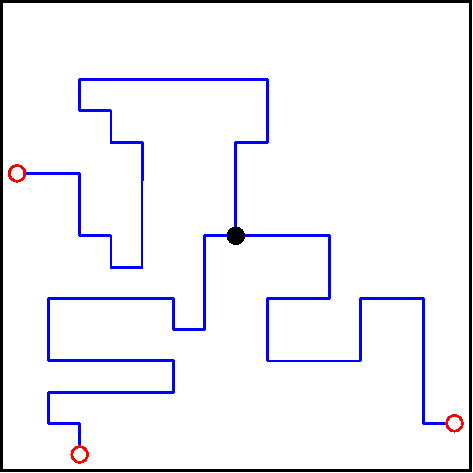
\includegraphics[width=0.95\linewidth]{img/SA final.pdf}
        \subcaption{Result ($t_{final} = 1$)}
    \end{minipage}
    \caption{Evolution of paths during simulated annealing.}
    \label{fig:simulated-annealing}
\end{center}

\subsection{Simplifying the Relative Improvement Calculation}\label{sec:analysis-proof-improvement}

In this section, we will show that the \emph{relative improvement} defined in paragraph~\ref{head:sa-cost-function} can be calculated very efficiently.
Formally, we want to show that $r_i = f(s) - f(s')$ for $s'$ obtained by changing tile $v$ in $s$ to $w$ can be calculated as
\begin{equation*}
    r_i = c_e(v) - c_e(w)  + 2 c_t(v,s) - 2 c_t(w,s) + 2c(w,v) - 2.
\end{equation*}

We start by substituting the definition for the cost function $f$.
\begin{align*}
    r_i & = f(s) - f(s')                                                                                                                 \\
        & = \sum_{t \in s} \left(c_e(t) + \sum_{u \in s} c(t,u) \right) - \sum_{t \in s'} \left(c_e(t) + \sum_{u \in s'} c(t,u) \right). \\
\end{align*}
Now we separate $v$ from $s$ and $w$ from $s'$.
\begin{align*}
     & = \sum_{t \in s} \left(c_e(t) + c(t,v) + \sum_{u \in s - v} c(t,u)\right) - \sum_{t \in s'} \left(c_e(t) + c(t,w) + \sum_{u \in s' - w} c(t,u) \right) \\
     & = \left(c_e(v) + c(v,v) + \sum_{u \in s - v} c(v,u)\right) + \sum_{t \in s - v} \left(c_e(t) + c(t,v) + \sum_{u \in s - v} c(t,u)\right)               \\
     & \ - \left(c_e(w) + c(w,w) + \sum_{u \in s' - w} c(w,u) + \sum_{t \in s' - w} \left(c_e(t) + c(t,w) + \sum_{u \in s' - w} c(t,u) \right) \right).       \\
    \intertext{We use that $s - v = s' - w$, and we name $q$ the set of tiles both states have in common.}
     & = c_e(v) + c(v,v) + \sum_{u \in q} c(v,u) + \sum_{t \in q} \left(c_e(t) + c(t,v) + \sum_{u \in q} c(t,u)\right)                                        \\
     & \ - \left(c_e(w) + c(w,w) + \sum_{u \in q} c(w,u) + \sum_{t \in q} \left(c_e(t) + c(t,w) + \sum_{u \in q} c(t,u) \right)\right)                        \\
     & = c_e(v) + c(v,v) + \sum_{u \in q} c(v,u) + \sum_{t \in q} c_e(t) + \sum_{t \in q} c(t,v) + \sum_{t \in q} \sum_{u \in q} c(t,u)                       \\
     & \ - \left(c_e(w) + c(w,w) + \sum_{u \in q} c(w,u) + \sum_{t \in q} c_e(t) + \sum_{t \in q} c(t,w) + \sum_{t \in q} \sum_{u \in q} c(t,u)\right)        \\
     & = c_e(v) + c(v,v) + \sum_{u \in q} c(v,u) +  \sum_{t \in q} c(t,v)                                                                                     \\
     & \ - \left(c_e(w) + c(w,w) + \sum_{u \in q} c(w,u) + \sum_{t \in q} c(t,w) \right).                                                                     \\
    \intertext{The function $c$ is symmetric, because it depends only on the distance between the tiles, which is symmetric, so we get:}
     & = c_e(v) + c(v,v) + 2 \sum_{t \in q} c(v,t) - \left(c_e(w) + c(w,w) + 2 \sum_{t \in q} c(w,t) \right).                                                 \\
    \intertext{The crowding a tile inflicts to itself is 1, so $c(v,v) = c(w,w)$.}
     & = c_e(v) - c_e(w)  + 2 \sum_{t \in q} c(v,t) - 2 \sum_{t \in q} c(w,t) .                                                                               \\
    \intertext{We can add the terms $2c(v,v) - 2c(v,v) + 2c(w,v) - 2c(w,v)$ because they sum to zero:}
     & = c_e(v) - c_e(w)  + 2 \sum_{t \in q} c(v,t) - 2 \sum_{t \in q} c(w,t)                                                                                 \\
     & \ + 2c(v,v) - 2c(v,v) + 2c(w,v) - 2c(w,v),                                                                                                             \\
    \intertext{and we collect the sums to sum over the elements of $s$:}
     & = c_e(v) - c_e(w)  + 2 \sum_{t \in s} c(v,t) - 2 \sum_{t \in s} c(w,t) - 2c(v,v) + 2c(w,v)                                                             \\
     & = c_e(v) - c_e(w)  + 2 c_t(v,s) - 2 c_t(w,s) - 2c(v,v) + 2c(w,v)                                                                                       \\
     & = c_e(v) - c_e(w)  + 2 c_t(v,s) - 2 c_t(w,s) + 2c(w,v) - 2 .                                                                                           \\
\end{align*}
$\hfill\square$

\subsection{Final Paths}

Now that we have generated the main paths, we just have to generate the side branches.
The world generation steps that come after have to make sure to not block the paths we have generated.
However, we don't want to constrain them with the whole path network.
Since we don't have requirements on the minimum side branch count or their lengths, it is enough to ensure the paths we generated in the previous step get preserved.
We can generate the rest of the world first, and only then make extra paths where they fit.
We don't want the branching to feel the same in every level.
This lets us use the randomness of the world generation instead of needing to introduce more in this stage.

This means, that this step will start with an already generated terrain and obstacles, as described in sections~\ref{sec:analysis-terrain-generation} and~\ref{sec:analysis-obstacles}.
These steps respect the original paths, but they will cause other tiles or edges between them to be blocked, as shown in figure~\ref{fig:paths-world}.
Here, we can see the original paths on the left.
On the right, we can see tiles blocked by obstacles as gray squares with black edges.
Additionally, some edges between tiles are also blocked, usually because the two tiles are at different height levels, separated by a cliff.
These are the remaining black lines.

\begin{center}
    \captionsetup{type=figure}
    \begin{minipage}{.5\textwidth}
        \centering
        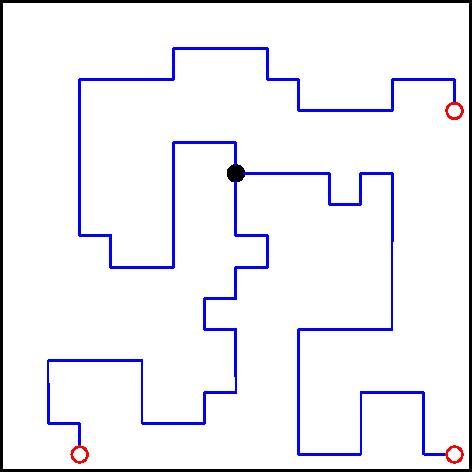
\includegraphics[width=0.95\textwidth]{img/Generated Paths.pdf}
    \end{minipage}%
    \begin{minipage}{.5\textwidth}
        \centering
        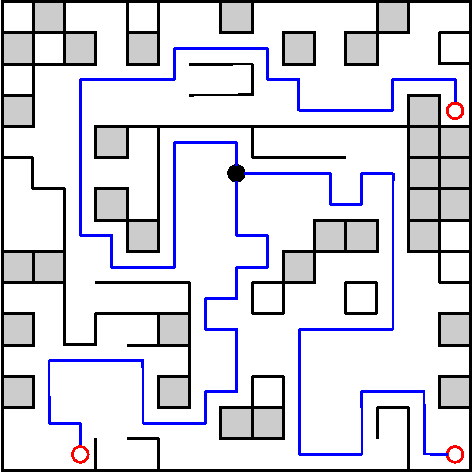
\includegraphics[width=0.95\textwidth]{img/Paths and world.pdf}
    \end{minipage}
    \caption{Blocked edges and tiles after generating the terrain and obstacles.}
    \label{fig:paths-world}
\end{center}


Now, how do we actually generate the path network?
There are so many blocked edges that we want to add all the valid branches we find, up to the maximum number of branches decided by the map generator (see section~\ref{sec:analysis-procedural-generation}).
To do this, we will use depth first search, but we will add a few heuristics to produce better paths.
To decide on these heuristics, we will set a few more requirements:
We still want the paths to be spread out, but we would prefer the paths to go straight if possible.

However, we would also like to somehow capture the shape of the paths that were optimized during the previous stage.
We could simply make the first path from each start be identical to the original path.
We would like multiple paths to sometimes join together, which we cannot do without changing them.
To achieve this, we add a rule for every tile with a path: if an original path also went through it, its path distance must be the same as the original path distance.
This way, the path segments of any new path will be distributed similarly to the original path, since they cross at every choke point.
This is illustrated in figure~\ref{fig:respect-originals}.
On the left are the original paths, and on the right are randomly generated paths which respect the rule.
The tiles where the random paths would intersect the original paths are marked with a blue circle.

\begin{center}
    \captionsetup{type=figure}
    \begin{minipage}{.5\textwidth}
        \centering
        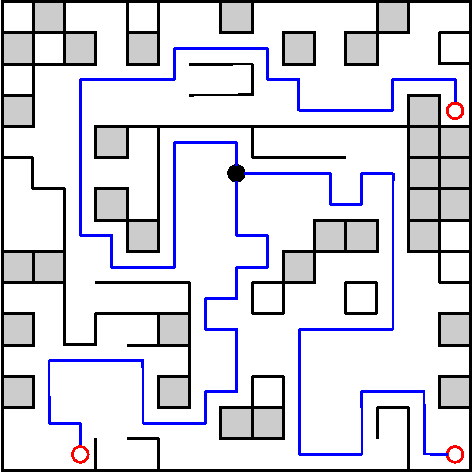
\includegraphics[width=0.95\textwidth]{img/Paths and world.pdf}
    \end{minipage}%
    \begin{minipage}{.5\textwidth}
        \centering
        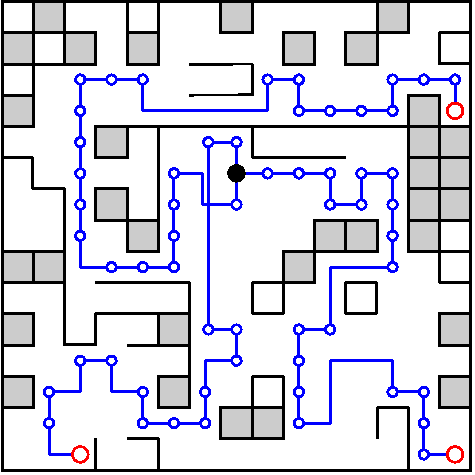
\includegraphics[width=0.95\textwidth]{img/Rnadom but respecting the originals.pdf}
    \end{minipage}
    \caption{Randomly generated paths which respect the original path distances.}
    \label{fig:respect-originals}
\end{center}

We need to make sure the paths we produce are the correct length and respect the required original path distances.
We can save a lot of time by precomputing the minimum distance each tile can have.
This way the algorithm can avoid tiles from which it's impossible to finish a path of the correct length.
For this, we can do a breadth first search from the Hub tile, and we restrict the original path tiles to only \enquote{be found} at the right time and not sooner.
The result can be seen in figure~\ref{fig:path-distances}.
We will call these distances the \emph{minimum distances}.

\begin{center}
    \captionsetup{type=figure}
    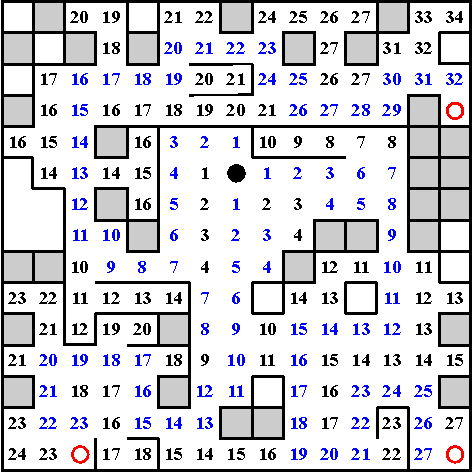
\includegraphics[width=0.5\textwidth]{img/Path Distances.pdf}
    \caption{Calculated minimum distances.}
    \label{fig:path-distances}
\end{center}

Now we finally run the depth first search, one path by one.
The algorithm keeps a stack of \emph{path prototypes}.
These are paths, which start at the start tile, but have not reached the Hub yet.
At the start, the stack contains only the path prototype with only the start position as its only element.
At every step, the algorithm pops the last prototype from the stack, finds all valid one-step continuations of the current paths, and adds those to the stack.

Valid continuations are the neighbors of the last tile of the current path prototype that aren't blocked.
Additionally, they have to have a minimum distance that is less than or equal to the remaining length of this path prototype.
The valid continuations are ordered such that the best option will be put onto the stack last, so it gets popped in the next step.
The best option is always the one that goes straight, and the rest is ordered by the same crowding penalty as in paragraph~\ref{head:sa-cost-function} of section~\ref{sec:analysis-our-simulated-annealing}.

Once the algorithm reaches the Hub or an already existing path, it checks whether it is valid to finish the current path.
First, it must have the correct remaining length to produce a valid path.
When it connects to the Hub, the remaining length must be 0, and for connecting to an existing path, the remaining length must match the path distance of that tile.
Additionally, as per requirement RP\ref{RP:branch}: \enquote{every branch must go through at least one tile that is not adjacent to any already existing path}.

If this check fails, the algorithm does not mark this branch, it pops the last item from the stack and continues from there.
If the check succeeds, it marks the new path section and updates the crowding penalties to take the new path section into account.
Then it continues by making another branch.

However, the last path prototype on the stack will share most of its tiles with the branch we just found.
We want the branches be separated from each other as much as possible.
To minimize the shared section, we take the path prototype from the opposite end of the stack.
So, in reality, we won't use a stack, but a double ended queue.
The entire search is described in pseudocode as algorithm~\ref{alg:path-finalizing}.

\begin{algorithm}[H]
    \caption{Finalizing paths}
    \label{alg:path-finalizing}
    \begin{algorithmic}[1]
        \ForEach{path start $start$}
        \State $stack$.\Call{PushLast}{path prototype containing only $start$}
        \State $success \gets$ \mono{false}
        \Statex
        \While{$stack$ is not empty}
        \If{$success$}
        \State $p \gets stack$.\Call{PopFirst}{}
        \Else
        \State $p \gets stack$.\Call{PopLast}{}
        \EndIf
        \Statex
        \If{last tile in $p$ contains a path or the Hub}
        \State $success \gets$ \Call{TryFinishPath}{$p$}
        \Else
        \State $success \gets$ \mono{false}
        \ForEach{tile $c$ from \Call{GetValidContinuations}{$p$}}
        \State $stack$.\Call{PushLast}{$p$ extended by $c$}
        \EndFor
        \EndIf
        \EndWhile
        \EndFor
        \Statex
    \end{algorithmic}
\end{algorithm}

With this ordering of valid continuations, the algorithm usually reaches the Hub too soon, and then it has to backtrack many times before producing a path that is the right length.
To fix this, we prioritize above all the tiles with minimum distance exactly equal to the remaining length.
The results of the algorithm are displayed on the right in figure~\ref{fig:final-paths}, compared to the initially generated paths on the left.
Segments that have changed are highlighted in red.

\begin{center}
    \captionsetup{type=figure}
    \begin{minipage}{.5\textwidth}
        \centering
        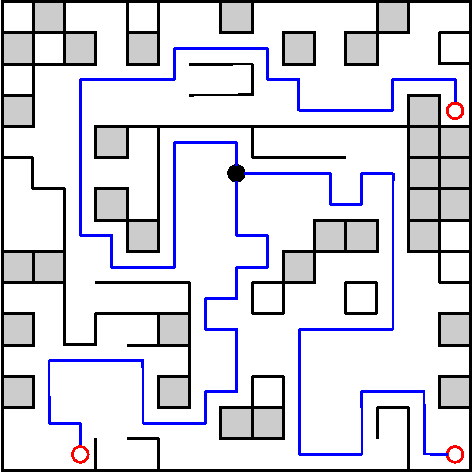
\includegraphics[width=0.95\textwidth]{img/Paths and world.pdf}
    \end{minipage}%
    \begin{minipage}{.5\textwidth}
        \centering
        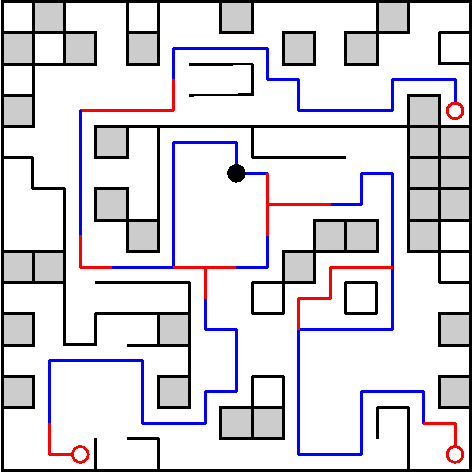
\includegraphics[width=0.95\textwidth]{img/Final Paths.pdf}
    \end{minipage}
    \caption{Final paths compared to the originally generated paths.}
    \label{fig:final-paths}
\end{center}

\section{Terrain Generation}\label{sec:analysis-terrain-generation}

There are many techniques we could use for generating the terrain.
However, we have pretty strict requirements for the terrain generation.
For example, we need to make sure the paths we have generated in the previous step are not blocked by terrain features like cliffs.

This led us to choose a variant of a procedural generation algorithm called \emph{model synthesis}, originally developed by \Citeauthor{ModelSynthesis}~\cite{ModelSynthesis}.
The discrete version of this algorithm is better known by the name \emph{wave function collapse} (or~WFC in short), popularized by \Citeauthor{WFC} on GitHub~\cite{WFC}.
Model synthesis is more general and focuses more on 3D models, whereas WFC applies the same concepts to generating 2D pixel art and tile maps.
Since the name \enquote{wave function collapse} is more popular, we will use it in the rest of this thesis, even though it's not the original name.

We chose WFC, because it can generate randomized terrain, whilst fully respecting the initial constraints we give it.
To see how this works, we will explain the algorithm first.

\subsection{Wave Function Collapse}

The original intent behind the algorithm is to replicate the structure of an example on a larger scale, making sure that the output is locally similar to the input, as shown in figure~\ref{fig:wfc-example}.
We will limit our examples to 2-dimensional grids of tiles, however this algorithm works in more dimensions, and even for irregular cells.

\begin{center}
    \captionsetup{type=figure}
    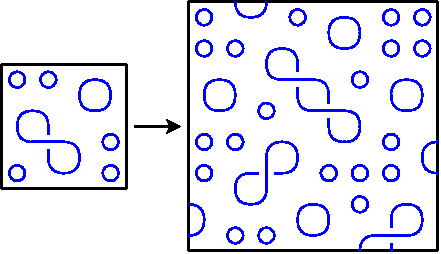
\includegraphics[width=0.5\textwidth]{img/WFC Example.pdf}
    \caption{Example input and output of the wave function collapse algorithm.}
    \label{fig:wfc-example}
\end{center}

The first step of the algorithm is to extract from the input which features can appear next to each other.
The algorithm creates a set of \emph{modules}\footnote{This is a naming convention used in an article by \Citeauthor{WFCMarian}~\cite{WFCMarian}.}, which are the building blocks the output will be built from.
Each module comes with a set of constraints on its neighbors.
The main portion of the algorithm then builds the output from these modules, such that all the constraints are satisfied, and each module appears in the output with a similar frequency to the input.
However, we will create the modules for our generator by hand, including their constraints, in order to have greater control over the generated result.
In figure~\ref{fig:wfc-modules}, we can see a set of 7 modules and the resulting output, given only the constraint that the edges of directly adjacent modules must match.

\begin{center}
    \captionsetup{type=figure}
    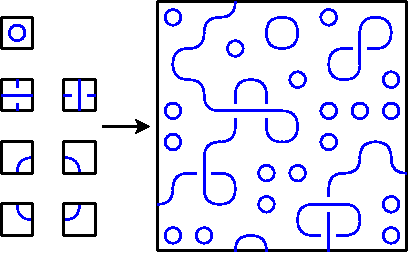
\includegraphics[width=0.5\textwidth]{img/WFC modules.pdf}
    \caption{Example output of WFC, using the modules on the left and only the constraint that their edges must match.}
    \label{fig:wfc-modules}
\end{center}

We call each spot in the output where a module is supposed to be a \emph{slot}.
Each slot keeps track of all the modules that can be placed in it.
At the start of the main part of the algorithm, all slots are initialized with all the modules.
Figure~\ref{fig:wfc-initial} shows a visualization of this state.
Then the algorithm repeats two actions: collapse a slot, propagate constraints.
To collapse a slot, the algorithm removes all possible modules from the slot except for one, chosen at random.

Then it has to propagate constraints, which means that it removes from each slot all the modules which can no longer be placed there.
For example, in figure~\ref{fig:wfc-step-1} we see that a slot has collapsed to a module which has a line on each edge.
Thus, the algorithm removes from the neighboring slots (marked in red) all modules which don't have a line at the corresponding edge.
After propagating constraints, the algorithm collapses another slot and so on.

\begin{center}
    \captionsetup{type=figure}
    \begin{minipage}{.31\textwidth}
        \centering
        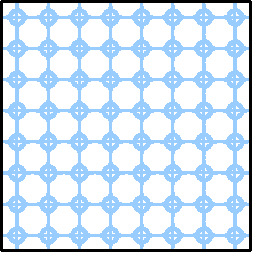
\includegraphics[width=0.95\linewidth]{img/WFC initial state.pdf}
        \subcaption{Initial state} \label{fig:wfc-initial}
    \end{minipage}%
    \begin{minipage}{.31\textwidth}
        \centering
        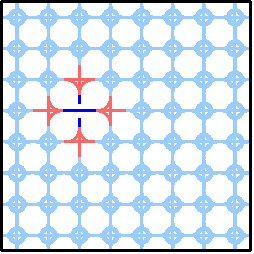
\includegraphics[width=0.95\linewidth]{img/WFC step 1.pdf}
        \subcaption{First step} \label{fig:wfc-step-1}
    \end{minipage}%
    \begin{minipage}{.31\textwidth}
        \centering
        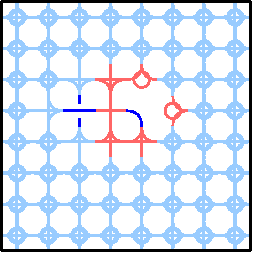
\includegraphics[width=0.95\linewidth]{img/WFC step 2.pdf}
        \subcaption{Second step} \label{fig:wfc-step-2}
    \end{minipage}
    \caption{Two steps of wave function collapse. Uncollapsed slots are drawn in light blue, uncollapsed slots that changed are drawn in red.}
    \label{fig:wfc-steps}
\end{center}

In figure~\ref{fig:wfc-step-2}, we can see an interesting situation after collapsing a second slot.
The slot between the collapsed slots can still contain two possible modules, however both of them have a line at the top and bottom edges.
This means that the algorithm also has to propagate to the neighbors of this tile that they have to have lines at the corresponding edges.
A change in one slot can affect slots even very far away from it.

This process repeats until all slots are collapsed, at which point we have successfully generated the output.
This process is summarized as algorithm~\ref{alg:wfc}.
We left out one detail: which element does \textsc{Pop} select?
This does not matter for the overall function of the algorithm, and it will be further discussed in section~\ref{sec:analysis-our-wfc}.
We will call this algorithm WFC, even though it differs from both WFC by Gumin and Merrell's model synthesis.
The only notable difference is that we skip the feature extraction step, and the algorithm takes as input the modules directly.

\begin{algorithm}[H]
    \caption{A na\"{i}ve version of wave function collapse}
    \label{alg:wfc}
    \begin{algorithmic}[1]
        \ForEach{slot $s$ in output} \Comment{Initialize all slots.}
        \State $s.modules \gets all\_modules$
        \EndFor
        \Statex
        \State $uncollapsed \gets$ all slots
        \While{$uncollapsed$ is not empty}
        \State $s \gets uncollapsed$.\Call{Pop}{} \Comment{Collapse a slot.}
        \State $s.modules \gets \{$random module from $s.modules\}$
        \Statex
        \State $to\_update \gets$ neighbors of $s$ \Comment{Propagate constraints.}
        \While{$to\_update$ is not empty}
        \State $u \gets to\_update$.\Call{Pop}{}
        \Statex
        \State $changed \gets$ \mono{false}
        \ForEach{module $m$ in $u.modules$} \Comment{Remove invalid modules.}
        \If{not \Call{IsValid}{$m$}}
        \State $u.modules \gets u.modules - m$
        \State $changed \gets$ \mono{true}
        \EndIf
        \EndFor
        \Statex
        \If{$changed$} \Comment{If $u$ changed, enqueue its neighbors.}
        \State $to\_update \gets to\_update\,\cup$ neighbors of $u$
        \EndIf
        \Statex
        \EndWhile
        \EndWhile
        \Statex
    \end{algorithmic}
\end{algorithm}

However, it is possible for the algorithm to create a slot with no valid module.
In that case, it is no longer possible to create a valid output.
We call this situation a \emph{conflict}.
An example can be seen in figure~\ref{fig:wfc-backtracking}.
If we look at WFC as a \emph{constraint satisfaction problem} solver, we can see that the constraint propagation only ensures \emph{arc-consistency}, which is not enough to rule out conflicts~\cite{LocalConsistencyWiki}.

We called algorithm~\ref{alg:wfc} na\"{i}ve, because it is unable to deal with any conflicts.
What can we do to always produce a result, even when a conflict happens?
One option is to simply restart the algorithm.
For sufficiently small outputs, this should be rare enough, only needing a few restarts.

Another option is to use backtracking.
Whenever the algorithm runs into a contradiction after collapsing a slot, it returns to the state before collapsing.
Additionally, it removes the module the slot collapsed to from its valid options, because it now knows it causes to a conflict.
The state after backtracking is illustrated in fig~\ref{fig:wfc-after-backtracking}.
This way, the algorithm can continue generating without getting rid of all its progress.

\begin{center}
    \captionsetup{type=figure}
    \begin{minipage}{.31\textwidth}
        \centering
        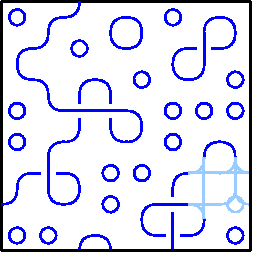
\includegraphics[width=0.95\linewidth]{img/WFC backtracking before.pdf}
        \subcaption{Before collapsing} \label{fig:wfc-before-backtracking}
    \end{minipage}%
    \begin{minipage}{.31\textwidth}
        \centering
        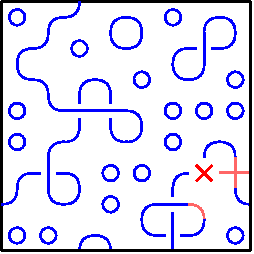
\includegraphics[width=0.95\linewidth]{img/WFC backtracking dead end.pdf}
        \subcaption{After collapsing} \label{fig:wfc-dead-end}
    \end{minipage}%
    \begin{minipage}{.31\textwidth}
        \centering
        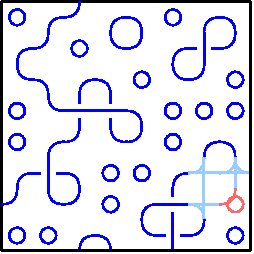
\includegraphics[width=0.95\linewidth]{img/WFC backtracking after.pdf}
        \subcaption{After backtracking} \label{fig:wfc-after-backtracking}
    \end{minipage}
    \caption{Conflicts and backtracking in WFC. The red cross marks a slot with no valid modules.}
    \label{fig:wfc-backtracking}
\end{center}

\subsection{Advantages and Disadvantages of WFC}

The main advantage of WFC is that it offers a lot of control over the generated world.
That's ultimately why we chose to use it.
We always know what features can appear in the world, because we explicitly allowed them to exist.
We can also freely constrain the world that we are generating.
For example, we can force the generator to not block the paths we've generated in the previous stage, and we can force the tile with the Hub to be flat.
We also force a random tile to be at the lowest height level and another to be at the highest.

However, WFC has some disadvantages when used as a terrain generator.
First, it can be very slow.
The time it takes algorithm~\ref{alg:wfc} to run scales linearly with the number of slots, which is not bad when we never run into contradictions.
Merrell shows in their thesis that deciding whether an incomplete output is consistent, i.e. it can be completed without running into contradictions, is an NP-complete problem.
This necessarily means that WFC isn't very fast in the worst case.

The real problem is that the algorithm usually does run into contradictions, and the larger the generation task, the more likely it is to run into a contradiction.
This is especially bad for online generation of infinite worlds, because we can't simply restart and generate a new world after the player has already seen a part of it.
Backtracking also doesn't solve this issue, because the algorithm can collapse a slot in a way that is guaranteed to cause a contradiction, and then do arbitrarily many more steps before finally running into it.
Of course, there are ways to circumvent this issue, namely by making the individual generation tasks smaller.
In their thesis, Merrell describes a technique called \emph{modifying in parts} based on this approach.

Another potential problem with WFC is that the individual slots or modules can be very apparent and repetitive.
This can be solved by procedurally generating the resulting geometry the player sees, only based on the modules chosen by WFC.
Another way to make the slots less apparent is to make the slots irregular.
Both of these techniques are used by \emph{Townscaper}~\cite{Townscaper}, a game by Oskar St\r{a}lberg.

Also, WFC only uses local constraints, so it provides no control over the more global features of the output.
On a large scale, the results are very homogenous.
For larger outputs, WFC should only be used to generate the local features, guided by large-scale features generated by some other algorithm.

Luckily, none of these disadvantages matter for our use case.
Our worlds are very small, and we don't mind that the tiles will be apparent, since the gameplay of our game is centered around them anyway.

\subsection{Using WFC for Terrain Generation}\label{sec:analysis-our-wfc}

Even though we want to generate a 3D terrain, our output will consist of a 2D grid of slots.
We want the tiles of the generated world to be at different heights, however, we don't want any tiles to generate above other tiles.
Ultimately, this is a 2D generation task, with the addition that modules can appear at different height levels.

At first, it might seem sensible to have one slot per world tile.
However, each tiles on it sown will be mostly a flat square.
The interesting terrain features will appear on the boundaries between the tiles.
For example, two tiles at different height levels next to each other will have a cliff separating them.
If we wanted to incorporate the cliff into the tile module, which tile does it belong to?
What about the features where the corners of four tiles meet?
We offset the slots in a way shown in figure~\ref{fig:tiles-and-slots}, such that each slot is responsible for four quarter-tiles of the world.
This way, the modules dictate how can the adjacent tiles connect to each other.

\begin{center}
    \captionsetup{type=figure}
    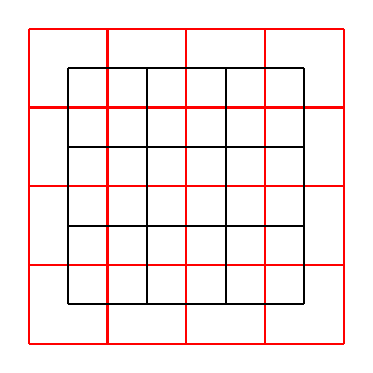
\begin{tikzpicture}
        \draw[step=1.0,thick,red] (0,0) grid (4,4);
        \draw[step=1.0,black,thick,shift={(0.5,0.5)}] (0,0) grid (3,3);
    \end{tikzpicture}
    \caption{The slots for generating a $3\times3$ tile world. Tiles are drawn in black, slots in red.}
    \label{fig:tiles-and-slots}
\end{center}

One example of such module is shown in figure~\ref{fig:wfc-module}.
Each module constrains the 8 adjacent slots.
An edge type is specified for each edge, and modules which share an edge must have the same edge type.
For each corner of the module, several tile constraints are specified.
The modules that share a tile must agree on the tile's properties: its height, slant direction (if any) and surface type.
Terrain types can have multiple surface types, each with a different set of modules and a few modules that allow to transition between them.
For example, a \emph{shore} module could have \emph{ground} tiles on one side and \emph{water} tiles on the other.
For each terrain type, it is also specified which surface types and which edge types block paths.

\begin{center}
    \captionsetup{type=figure}
    \begin{minipage}{.5\textwidth}
        \centering
        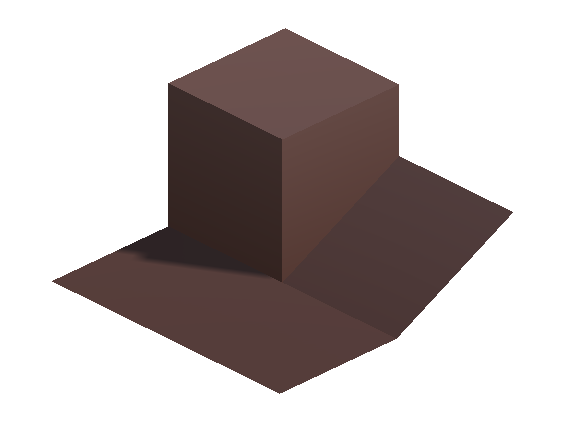
\includegraphics[width=0.95\textwidth]{img/Module model.png}
    \end{minipage}%
    \begin{minipage}{.5\textwidth}
        \centering
        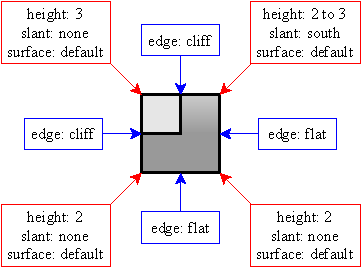
\includegraphics[width=0.95\textwidth]{img/Module constraints.pdf}
    \end{minipage}
    \caption{An example module and its constraints.}
    \label{fig:wfc-module}
\end{center}

In figure~\ref{fig:wfc-modules}, we show 7 modules as an input.
However, when designing them, it would make more sense to think of them as 3 different modules that can each be rotated.
Thus, the modules we use will also have an option to select the allowed reflection and rotations.
Then, before generating the terrain, we will automatically generate all variants of each module.
Each module can also be placed at different height levels, which is handled similarly.
For example, the module shown in figure~\ref{fig:wfc-module} will effectively become 24 different modules in a terrain type with 4 height levels (0, 1, 2, 3), because it has 8 different reflections and rotations, and it can appear at 3 different height levels (0--1, 1--2, 2--3).

For each module, we also specify a weight.
This dictates how likely it is to be selected when collapsing a slot, compared to other modules.
For example, when we collapse a slot that only has two valid modules, with weights 1 and 4, then the first module will be selected with a 20\,\% probability.

We have decided to implement backtracking to solve contradictions.
If the algorithm only ever has to backtrack once before collapsing another slot, we say that it needs backtracking depth 1.
However, it is possible that the algorithm collapses a slot, finds a contradiction, and after backtracking, removes the only remaining module in the slot that was collapsed.
Thus, it creates another contradiction, which causes it to backtrack deeper.

We ran some quick tests with the set of modules which is going to be used to generate terrain in the demo version.
During these tests, we were unable to generate a single world, without running into a contradiction.
However, most worlds only ever needed backtracking depth of 1 to successfully generate.
After that, we ran into diminishing returns.
Of the worlds that required backtracking depth 2, most required backtracking depth greater than 10.
So we decided to allow for backtracking depth 1 and otherwise just restart the generation, which makes it faster on average.

\xxx{I should probably provide the exact data I measured. Do I also need to explain the whole setup to make it reproducible?}

We also need to decide which slot to collapse at each step of the algorithm.
Merrell uses in their thesis a sort of scan line order, collapsing them in the lexicographic order of their coordinates.
This could theoretically introduce a directional bias in the results.
Gumin in their implementation always collapses a slot with the lowest \emph{Shannon entropy}.
This causes the generation to collapse slots outwards form the slot that was collapsed first.
From our testing, the results tend to look unnatural, often creating rectangular regions at the same height, or repeating patterns.

Both of these orders grow the collapsed portion of the world from one initial slot, similar to growing a regular crystal from one seed crystal.
To make the results more natural, we chose to select the slot to collapse at random.
This leads to the generator first collapsing slots in various parts of the world to different configurations.
Then it has to somehow connect these to make the world follow the rules we set.
This leads to more diverse results, however, the failure rate becomes very high, leading to slower generation.

As a compromise, we chose to weight the slots by the number of invalid slots\,$+\,1$.
This is an approximation of entropy that is trivial to compute, making it more likely to select more constrained slots, but still collapsing unconstrained slots once in a while.
The 1 is added just to make all weights nonzero.
This leads to results similar to the ones with uniform randomness, but decreases the failure rate substantially.

\xxx{More testing data to compare the success rate of the different approaches}

\xxx{A picture of the result?}

\section{Resources and Obstacles}\label{sec:analysis-obstacles}

- after terrain generation, place blockers on tiles

- materials for the player to mine

- just rocks for variety - the player cant build on these

- set up as a few layers

- each stage has:

- one or more types of blocker (e.g. ore, small rocks, big rocks)

- *min* and *max* amounts

- *base chance* to place

- whether they can be placed on slanted tiles

- which surface Types they can be on (currently there is only one)

- *forces* - effect on chance based on already placed blockers

- for example: negative force with magnitude *m* from stage *s* means the chance to place a blocker on a given tile is decreased by *m/d*  for each blocker placed in stage *s*, where *d* is its distance from the considered tile

- for each stage:

- repeat until at least min blockers have been placed (in this stage)

- for each tile without a path or blocker (in random order):

- if random number between 0 and 1 < modified chance:

- place the blocker of the given type

- if there are max blockers (placed in this stage), end the stage

- scattering models

- unity physics engine X

- parallel

For the blockers, I didn't want repetitive obstacle models, so they are generated proceduraly by scattering many simpler models (decorations) on each tile

- first compute weights based on various factors (images!!!)

- distance to path

- height

- distance to other blockers

- customizable thanks to modular approach

- then scatter decorations in stages, each stage again having one type of decoration and many parameters

- for each tile in random order repeat x (specified for this stage) times:

- pick a random position within it

- calcualte the weight at this position (based on settings)

- check that it is greater than some threshold (based on settings)

- calculate the minimum distance to other decorations (from weight, based on settings)

- check that the position is far enough from other decorations

- calculate the decoration size (from weight, based on settings)

- place the decoration on this position, with the given size

\section{Terrain Types}

- what information is tied to the type

- why txt (inspector was not as legible)

\section{World Builder}

- builds the world from the generated data, it needs to be done in the main thread

- the rest will be in background threads

\section{Attacker Wave Generation}\label{sec:analysis-waves}

- creates a randomized plan of waves

- two types of waves

- combine different attackers in sequence

- combine different attackers in parallel (only possible with multiple paths, rarer)

- each wave gets some throughput budget and buffer

- each attacker has a given cost

- when planning a wave, select attackers and spacing, such that the througput budget is exceeded

- for each attacker subtract the throughput overshoot from buffer

- fit such that as much of buffer gets used without going over

- branching

\section{Simulation}

- use fixed updates for game logic

- why?

- 20Hz = fixed time step 0.05s

- options to speed up or possibly pause - changing fixed update rate - not yet implemented

\section{Visuals and Interpolation}

- interpolate positions and visuals on Update

- many visuals are game-speed agnostic     - TODO: use unscaledDeltaTime

- I thought about some custom mini-framework for this, but many of the simulated variables the visuals are based on should be handled on case-by-case basis

\section{Attacker Targeting}

- Towers use it to acquire targets

- handles which Attackers are in range and which one is chosen as the current target

- can require line of sight to the enemy

- different targeting types

- rotation

- heights

- possibly ensure a trajectory

- preferred target (configurable)

- composite colliders

\section{Range Visualization}

- IMAGES!!

- Draw the range on the terrain mesh

- Draw on which parts of paths will Attackers be targeted

- green - all sizes

- yellow - only large

- Terrain shader uses compressed texture format instead of raw texture

- Options:

- quadrant compression format, 2bytes per node

- less CPU time, because the data is already in this format

- up to 48KiB per frame

- more GPU time

- 256x256 texture, 1byte per pixel

- more CPU time

- 64KiB per frame

- fast on GPU

- only 1 channel - cannot interpolate

- mipmaps -> one additional state

- less CPU time

- 33\% more data

- more pixels per byte

- possible future optimization

- less data

- more difficult indexing and stuff both on CPU and GPU

- interpolation could work with more than one channel and without mipmaps

\section{Game Commands}

- we want various components to modify how other components function

- examples

- also react to events as a bonus

\section{Blueprints}

- separation of stats from behavior

- why are they implemented this way

\subsection{Attacker Stats}

- blueprints for attackers

\subsection{Dynamic Descriptions}

- explain what things do and their stats

- attackers and blueprints

- dynamically reflect the changes made by other components

\section{Random Number Generators}\label{sec:analysis-rng}

Randomized algorithms, like the ones we will use for procedural generation, depend on a \emph{random number generator} as their source of randomness.
A \textbf{random number generator} (or \emph{RNG}) produces a sequence of numbers that looks random and is unpredictable.
They are well explained in \citetitle{johnston2018random}~\cite{johnston2018random} by David Johnston.
Some RNGs use specialized hardware to generate truly random data using an external source of entropy, these are called \emph{true random number generators}.
However, we want a \emph{deterministic RNG}, also known as a \emph{pseudorandom number generator} (\emph{PRNG}).
These produce the random data using a completely deterministic algorithm, but unless we know the current internal state of the generator, the outputs still can't be predicted.
The initial state of a PRNG is called the \emph{seed}, and a generator will always generate the same sequence of outputs when \emph{seeded} with the same value.

Each query advances the generator's state, so the value a deterministic random number generator returns depends on the number of previous requests.
If we used one generator for generating everything, the outcomes of different systems would depend on the order they were generated in.
For example, when a player triggers some effect that uses randomness \emph{before} generating a level, the level would be different than if the player triggered the randomized effect \emph{after} the level was generated.
To remedy this, we will utilize a simple trick we call \emph{seed branching} all throughout the procedural generation.
Whenever we want more systems to be independent of each other, we create a new RNG instance for each system, and we seed them with each with a seed generated from the old RNG in advance.
For example, we will have a master RNG seeded with the seed of the run, from which we will generate the seeds for the map generator, reward systems, etc.
The map generator itself will generate the run map and then assign a new seed to each of the levels planned on the map, and so on.

We can determine what properties are required of the RNG we are going to use from our use-case.
First, obviously, the numbers generated by the generator should be random enough.
However, the RNG doesn't have to be cryptographically secure or pass strict statistical tests, since we aren't going to use them for cryptography or scientific simulations.
Since we will create many instances of the RNG, it should be lightweight and fast to initialize.
Some of them, for example the ones used by the reward system, will persist throughout the whole run, so we need an easy way to save the RNG's current state.
So, what options do we have?

Since we are using Unity, the first RNG that comes to mind is Unity class \mono{Random}~\cite{UnityRandom}.
It is designed to be easy to use, but it is very limited~--- for example, we have access to only one instance of the class and the same instance is used for other systems within the game engine.
This is a dealbreaker for us, because we want to create more instances, and we want to have complete control over them to ensure determinism.

Another option that's on-hand is .NET \mono{System.Random}~\cite{SystemRandom}.
According to the documentation, instantiating a random number generator is fairly expensive.
Furthermore, there are no methods to read and set the internal state of the generator.
This becomes a problem when we want to save the state of an instance to restore it later, for example when loading a save file.
We would have to serialize and deserialize the instance, which isn't a big problem, but it feels inelegant and inefficient.

Instead, we chose to go with a more straight-forward option~--- making our own RNG.
This way, we can make the generator have all the features we need.
There are many algorithms a PRNG can use.
Johnston describes in their book~\cite{johnston2018random} some most commonly used non-cryptographic PRNGs, namely:
\begin{itemize}
    \item Linear congruential generators (LCG),
    \item Multiply with carry (MWC),
    \item XORSHIFT,
    \item Permuted congruential generators (PCG).
\end{itemize}
All of these are random enough for our use-case, provided we use the right parameter values, so we chose an LCG, because it seemed the most simple to implement.
In the article \citetitle{LCGTables}~\cite{LCGTables}, the author explains the statistical tests they used to measure the randomness of the LCGs and tabulates the best-performing parameter combinations.
From there we took the parameters for our LCG implementation.